\documentclass{beamer}

\usetheme{CambridgeUS}
\usecolortheme{beaver}
\usenavigationsymbolstemplate{}
\usepackage{hyperref}
\usepackage{graphicx}


\title[ORM Inheritance]{Exploring ORM Inheritance}
\author{Collin Price}

\begin{document}

\begin{frame}
	\titlepage
\end{frame}

\section{Introduction}

\begin{frame}
	\frametitle{Object-Relational Mapper(ORM)}
	\begin{itemize}
		\item Database Abstraction Layer
		\item Lets you query and manipulate data from a database using an object paradigm.\
		\item Abstracts SQL statements.
		\item Can maintain model relationships in code.
	\end{itemize}
\end{frame}

\begin{frame}
	\frametitle{Composition Design}
	\begin{figure}
		\centering
		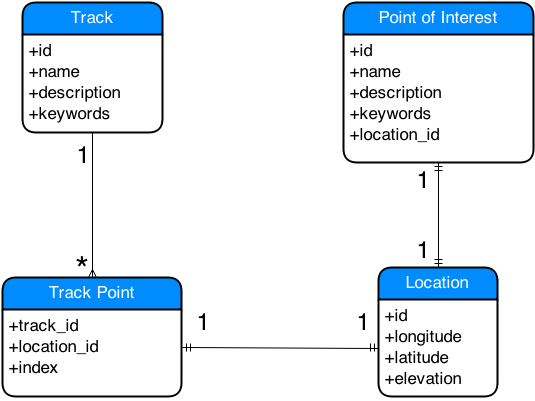
\includegraphics[scale=0.4]{resources/verbose-gps.png}
	\end{figure}
\end{frame}

\begin{frame}
	\frametitle{Inheritance Design}
	\begin{figure}
		\centering
		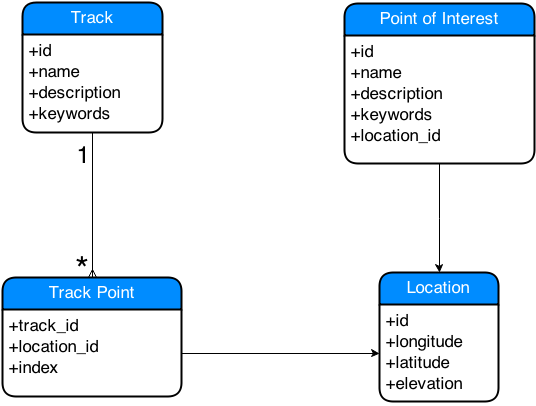
\includegraphics[scale=0.4]{resources/concise-gps.png}
	\end{figure}
\end{frame}

\section{Entity Framework}

\begin{frame}
	
	\begin{center}
		\Huge Entity Framework
	\end{center}
	\begin{center}
		ORM for .NET Framework
	\end{center}

\end{frame}

\begin{frame}
	\frametitle{Inheritance Types}
	
	\begin{itemize}
		\item Table-per-Type (TPT) inheritance
		\item Table-per-Hierarchy (TPH) inheritance (default)
		\item Table-per-Concrete Class (TPC) inheritance
	\end{itemize}

\end{frame}

\begin{frame}
	\frametitle{Table-per-Type (TPT) inheritance}
	\begin{figure}
		\centering
		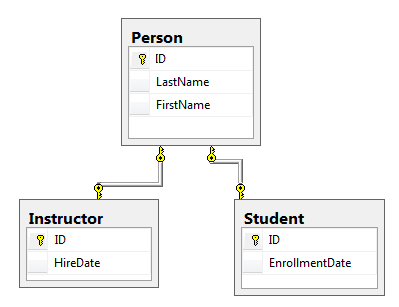
\includegraphics[scale=0.5]{resources/entity-framework/tpt.png}
	\end{figure}
\end{frame}

\begin{frame}
	\frametitle{Table-per-Hierarchy (TPH) inheritance}
	\begin{figure}
		\centering
		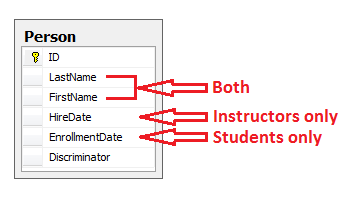
\includegraphics[scale=0.8]{resources/entity-framework/tph.png}
	\end{figure}
\end{frame}

\begin{frame}
	\frametitle{Table-per-Concrete Class (TPC) inheritance}
	\begin{figure}
		\centering
		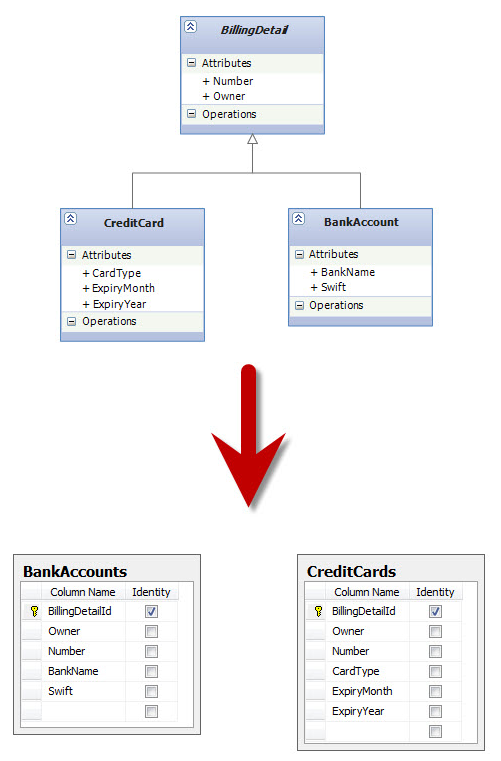
\includegraphics[scale=0.28]{resources/entity-framework/tpc.png}
	\end{figure}
\end{frame}

\section{Rails Active Record}

\begin{frame}
	
	\begin{center}
		\Huge Ruby on Rails: Active Record
	\end{center}

\end{frame}

\begin{frame}
	\frametitle{Single Table Inheritance (STI)}
	\begin{figure}
		\centering
		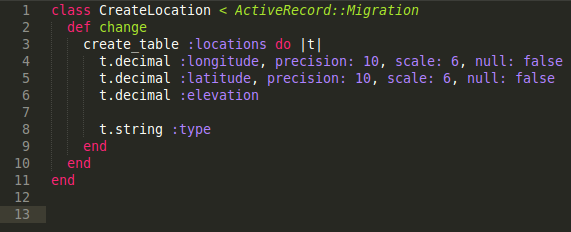
\includegraphics[scale=0.5]{resources/rails/migration.png}
	\end{figure}
\end{frame}

\begin{frame}
	\frametitle{Single Table Inheritance (STI)}
	\begin{figure}
		\centering
		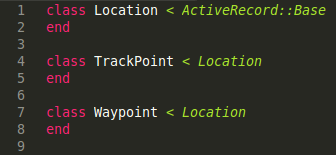
\includegraphics[scale=0.6]{resources/rails/classes.png}
	\end{figure}
\end{frame}

\begin{frame}
	\frametitle{Single Table Inheritance (STI)}
	
	\begin{itemize}
		\item Useful for tables with same fields but different behaviours.
		\item Unable to add additional fields to subclasses.
	\end{itemize}
\end{frame}

\section{Others}

\begin{frame}
	\frametitle{Hibernate (Java)}
	
	\begin{itemize}
		\item Table-per-Hierarchy (TPH) inheritance
		\item Table per Type (TPT) inheritance
		\item Table-per-Concrete Class (TPC) inheritance
	\end{itemize}

\end{frame}

\begin{frame}
	\frametitle{Eloquent (Laravel 4)(PHP)}
	
	\begin{itemize}
		\item Can manually create Single Table Inheritance support.
		\item http://snooptank.com/single-table-inheritance-with-eloquent-laravel-4/
	\end{itemize}
\end{frame}

\section{Conclusion}

\begin{frame}
	\frametitle{Discussion}
	
	\begin{itemize}
		\item Composition vs Inheritance
		\item Does inheritance belong in the database?
		\item Is the Don't-Repeat-Yourself principle violated with similar tables?
	\end{itemize}

\end{frame}

\begin{frame}
	\Huge{\centerline{Questions?}}
\end{frame}

\end{document}